\part{Analyse de l'existant}


\section{Fonctionnement de l'application Royal}

\subsection{Introduction}
Nous n'avions pas d'existant imposé à proprement parler, cependant nous avons été guidés vers Royal, un projet existant réalisé par des étudiants du département informatique de l'an passé.
Il apparait être une des solutions actuelles la plus en accord avec la demande du client, à savoir, de manière générale : « la gestion d'une bédéthèque ».

De ce fait, cet article traitera du fonctionnement de Royal.
C'est une application 
libre \footnote{Selon les termes de la GNU Lesser General Public License}
issue d'une amélioration de \emph{Birdy}, une autre application libre de gestion de livres.

\subsection{Aspect fonctionnel de Royal}
Royal permet la saisie d'informations sur une bande dessinée, tel que son titre, son auteur, son image de couverture (recherchée sur internet), sa date de parution, etc..
Il permet d'obtenir une liste de l'ensemble des \emph{BDs}, que l'on peut trier selon divers critères et réorganiser selon des collections de \emph{BDs}.
Royal permet l'enregistrement de \emph{BDs}, mais aussi d'informations concernant les auteurs ou encore les collections.

On peut aussi importer un ensemble de \emph{BD} à partir d'une base de données existante.
De plus, Royal intègre un système multi-lingues concernant son interface utilisateur, ainsi que d'une bibliothèque d'aide d'utilisation.

Après cette brève description de Royal, on peut observer que son utilisation permet déjà de répondre à plusieurs fonctionnalités décrites auparavant. 

\subsection{Aspect technique de Royal}
Royal est développé en Java et utilise la bibliothèque \emph{Swing} pour son environnement graphique. 
Le projet a été développé sous Linux, mais reste néanmoins exécutable sous d'autres systèmes d'exploitation comme Windows 7 par exemple, avec plus ou moins de succès. 
Le stockage des données est réalisé avec \emph{Hibernate}, c'est une structure gérant la persistance des objets en base de données. 
C'est un outil lourd et complexe, mais très puissant que nous allons ré-utiliser étant donné son existence sous Royal. 
Il permet un transfert simplifié entre les objets java et les bases de données.

\subsection{Analyse de la base de données}

Comme nous pouvons l'observer, le MCD existant traite un certain nombre d'éléments nécessaires pour l'enregistrement des informations de notre livre.
Les tables « Emprunteur » et « Location » ne sont actuellement pas utilisées dans Royal mais pourrait nous permettre d'enregister la date de retour et le lieu d'emprunt.
Néanmoins, des tables devront être ajoutées afin de rendre possible la sauvegarde d'informations concernant les bibliothèques.


\begin{figure}[hp]
 \centering
 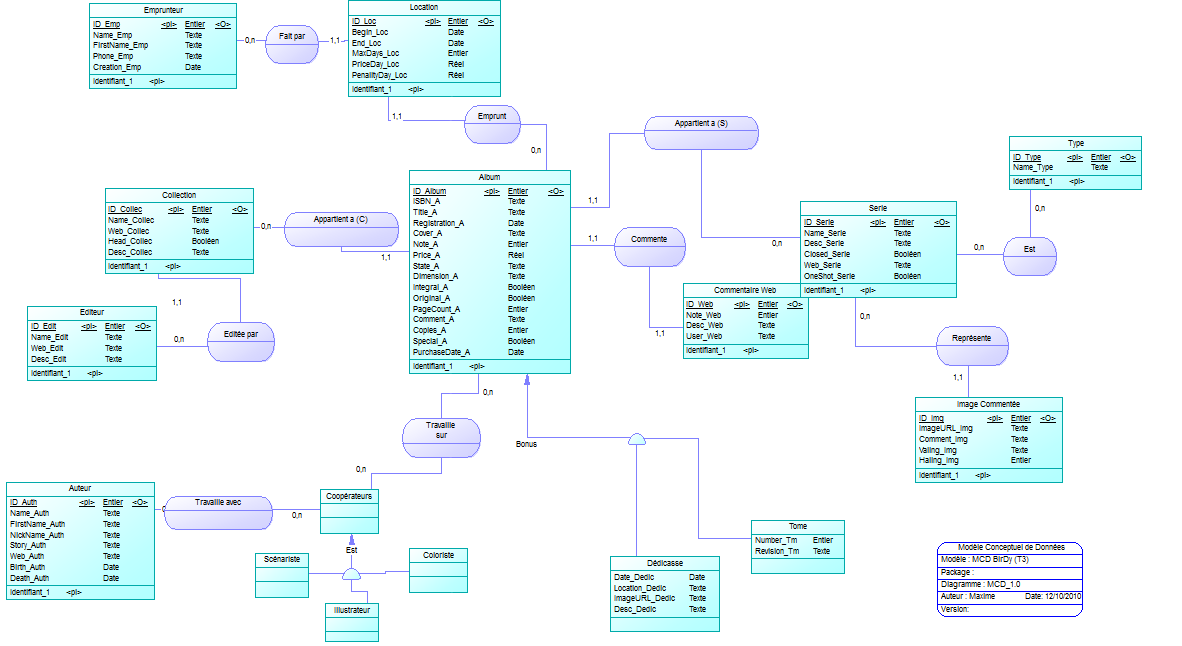
\includegraphics[height=24cm]{../img/MCD_Royal.png}
 % MCD_Royal.png: 646x1182 pixel, 96dpi, 17.09x31.28 cm, bb=0 0 485 887
\end{figure}

